\section{Discussion} % (fold)
\label{sec:discussion}
In this section we will look back at the problem introduced in section \ref{sec:introduction} and evaluate the implementation of Raft. This will be done by comparing our test results with the requirements stated in section \ref{sec:requirements}. Doing this, we can reflect on the overall goal of the project i.e. to gain deeper knowledge of Raft. Further extensions and improvements to the end product will then be proposed and discussed.

\subsection{Reflection on goal}
The goal of this project was to learn about what is the state of the art in terms of solving the consensus problem. In order to do this, our approach was to gain knowledge about Raft through implementing it in a simulated environment.
The requirements for the implementation stated that it should provide a tool for visualising the behaviour of Raft. \\
We divided our tests into white- and black box tests in order to document our development process better by testing the behaviour in the white box tests and come with example tests when verifying the solution itself in the black box tests. But the black box tests do not verify the correctness of the implementation, since they do not cover to whole space of possible scenarios. Another way to verify our implementation would have been to use a formal verification tool such as SPIN, which is used for testing models of concurrent systems. But this would require us to develop a whole new solution in another language i.e. Promela which conflicts with our main goal, which was to utilize the flexibility and small over head provided by Javascript. And in terms of the correctness of the implementation of Raft, referring back to the properties for non-Byzantine failure tolerant systems listed in section~\ref{sec:introduction}, the choice of platform again provides a poor basis for a formal verification. But it can be argued that by adopting the behaviour specified in the Raft paper thus also the safety properties, that our implementation upholds to properties of validity and integrity in the cases we have chosen to test.

\subsection{Experiences}

The biggest challenge of implementing the Raft algorithm is to implement and test the situations in parallel (such as mentioned with log replication and RPC's in elections) and the leader election driven by a randomly initialized timer.

In the situations in parallel we have suggested the method of using a protocol supporting both direct and delayed communicating between servers in section~\ref{sub:requestvote_rpc}. This made it easy to test the behaviour involving RPC's, but there are challenges in parallel computing that cannot be hidden with abstractions. The first one is race conditions which we experienced in the simulation when the RPC delay is to high in relation to the heartbeat interval. If the leader e.g. replicates a log entry $x\rightarrow5$ to a follower and before the follower is able to respond to the RPC (e.g. because of latency) a new hearbeat interval is started and the leader blindly tries to replicate the same log entry with $x\rightarrow5$. This will make the follower append the same entry twice. The situation is illustrated in figure~\ref{fig:replication_race_condition}. Although we discovered this implementation issue it did not ruin the consensus due to the safety rules of Raft and the problem was fixed by making the log appending method of followers idempotent as described in section~\ref{sub:log_replication_implementation}.

\begin{figure}
\centering
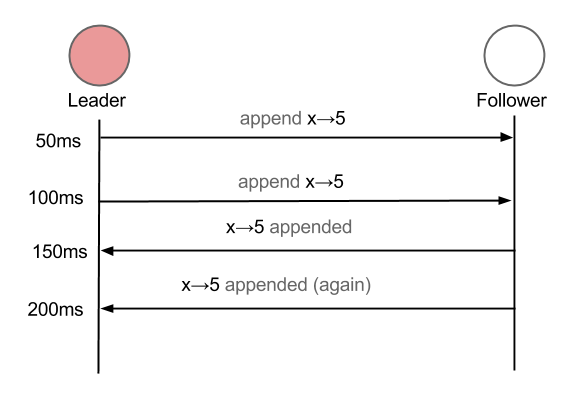
\includegraphics[scale = 0.5]{figures/replication_race_condition.png}
\caption{A situation with possible race condition when idempotent log appends is not implemented. This figure illustrates that some situations are only present when in parallel (or asynchronous).}
\label{fig:log_replication_implementation}
\end{figure}

\subsection{Further work}

% Using random election timeout and trouble with testing.
One of the problems with using a random election timer is that it is hard to test because of it is not possible to assert a random result. It would be possible to assert a property of the whole system such as ``There is only one leader after x seconds''. But the fact that the test have to be delayed several milliseconds make the tests slow and thereby slows down the development flow.

% - Hvordan gik det?
% - Hvad var svært?
% - Hvad kunne vi gøre bedre?
% - Future improvements?

% Hard to test parallel algorithms
%   - Raft uses randomized timers -> as explained - hard to test random stuff
%   - We tried to solve with protocol, but:
%     - This does not necessarily apply to the resulting parallel implementation
%     - Name the idempotent thing
%   - One missing point:
%     - index should be a part of the log entry
%       -  we used index in array - not correct
%

    %Det har været et problem at teste randomness, hvilket har været en udfordring.
% section discussion (end)
